\section{The benchmark loop}
\label{app:loop}

\begin{figure}[htbp]
\centering
\resizebox{0.70\textwidth}{!}{%
\begin{tikzpicture}[
  font=\small,
  box/.style={draw=black!55, rounded corners=2pt, align=center, inner sep=4pt,
              minimum height=9mm, text width=30mm},
  ag/.style={box, fill=blue!6,   draw=blue!60},
  sv/.style={box, fill=orange!8, draw=orange!70},
  ev/.style={box, fill=green!8,  draw=green!45!black},
  dl/.style={box, fill=black!4},
  fl/.style={-{Stealth[length=2mm]}, draw=black!70, thick},
  lb/.style={font=\scriptsize\itshape, text=black!60},
  hd/.style={font=\scriptsize\bfseries, text=black!70},
]

% ---- left: inside the evaluated cell ----
\node[dl] (task)  at (0,0)      {frozen task spec\\[1pt]{\scriptsize 5 parameters $\cdot$ solve budget\\ process gates}};
\node[ag] (agent) at (0,-2.1)   {agent harness\\[1pt]{\scriptsize \Ltwo{} library-assisted\\ \Lthree{} from scratch}};
\node[sv] (solv)  at (5.4,-2.1) {TokaMaker\\[1pt]{\scriptsize \GS{} FE solver}};
\node[dl] (deliv) at (0,-4.6)   {deliverable\\[1pt]{\scriptsize \code{report.json}\\ \code{predict.py}}};

\draw[fl] (task) -- (agent);
\draw[fl] ([yshift=3.5mm]agent.east) -- ([yshift=3.5mm]solv.west)
      node[midway,above,lb]{params};
\draw[fl] ([yshift=-3.5mm]solv.west) -- ([yshift=-3.5mm]agent.east)
      node[midway,below,lb]{$\psi$ or failure};
\draw[fl] (agent) -- (deliv);

\node[lb, text width=36mm, align=center] at (5.4,-3.2)
     {$\le 450$ solves, 3 adaptive rounds};

% ---- separator ----
\draw[dashed, black!45] (7.7,1.0) -- (7.7,-5.5);
\node[hd, anchor=south] at (2.7,0.85) {inside the evaluated cell};
\node[hd, anchor=south] at (10.9,0.85) {independent evaluation};

% ---- right: evaluation the agent never sees ----
\node[ev] (gates) at (10.9,-0.4) {contract gates\\[1pt]{\scriptsize did it deliver?}};
\node[ev] (score) at (10.9,-2.5) {frozen test set\\[1pt]{\scriptsize 60 held-out solves\\ relative $L_2$}};
\node[ev] (diag)  at (10.9,-4.6) {diagnostics\\[1pt]{\scriptsize valid? honest?}};

\coordinate (bus) at (8.6,-4.6);
\draw[fl] (deliv.east) -- (bus);
\draw[fl] (bus) -- (diag.west);
\draw[fl] (bus) |- (score.west);
\draw[fl] (bus) |- (gates.west);

\end{tikzpicture}%
}
\caption{The benchmark loop. The agent must \emph{buy} its own training data from
an expensive \GS{} solver under a fixed budget, choosing where to sample across
three adaptive rounds, and emits a deliverable that is checked, scored and
diagnosed entirely outside the cell on a test set it never sees. Every
condition passes through the identical right-hand column.}
\label{fig:loop}
\end{figure}


\section{Reproducibility}
\label{app:repro}

{\small
\begin{verbatim}
pip install -e ".[ml,dev,harnesses]"
python -m autotokamak.bench freeze-testset   # ground truth (committed)

tools/campaign_guard.py preflight --harnesses "ursa dspy pi cursor" \
                        --task benchmarks/tasks/L3_mini_v3.yaml
tools/run_campaign.sh --tag <tag> --reps 5 --parallel 6 --budget-usd 250 \
                      --harnesses "ursa dspy pi cursor"

python tools/cost_report.py        --tag <tag>
python tools/aggregate_matrix.py   --tag <tag>   # main table + all three tests
python tools/render_paper_figures.py --tag <tag> --out <paper>/figures
python tools/render_paper_tables.py  --tag <tag> --out <paper>/tables

python tools/run_library_baseline.py --n-samples 450 --seeds 0 1 2   # the L0 arm
python tools/run_control_arm.py      --reps 4                        # Section 7.4
python tools/judge_code.py score --tag <tag> --judge-provider openai \
                                 --samples 3 --per-cell 3            # Section 7.3
\end{verbatim}
}

Task texts are frozen and versioned; every run records the task's SHA-256, its
prompt version, its model string, and its replicate index. The frozen test set
carries provenance attributes (solver version, parameter and grid hashes,
scoring epoch) and is never regenerated. The statistics are seeded
(bootstrap and both permutation tests use seed \code{20260917}, 10\,000 and
20\,000 resamples respectively), so the analysis reproduces exactly from the
archived runs. Every figure and appendix table in this paper is generated from
those artifacts by the two scripts above rather than transcribed.

The one thing that does \emph{not} reproduce exactly is the agent runs
themselves: they are stochastic, and the substrates are versioned third-party
software that moves. That is why the campaign is replicated and reported with
intervals rather than as point estimates.

\section{Benchmark documentation}
\label{app:datasheet}

\paragraph{Access and hosting.}
The benchmark---task specifications, the deliverable contract, the frozen
evaluation assets, all harness adapters and every analysis script---is at
\url{https://github.com/hindyros/autotokamak}. The results in this paper are from
the campaign tagged \code{matrix-v4-20260919} at commit \code{dbc8289}. An
archival DOI is to be minted at camera-ready from the release tag.

\paragraph{Licensing.}
The benchmark code and task specifications are MIT licensed. The ground-truth
solver, Open FUSION Toolkit / TokaMaker \citep{hansen2024tokamaker}, is LGPL and
is used as an unmodified library dependency, which MIT-licensed code may do; we
redistribute no part of it. The frozen test set is derived data produced by that
solver from parameter vectors we generated, and is released under the same MIT
terms as the rest of the benchmark.

\paragraph{Maintenance.}
The contract, the evaluation grid and the frozen test set are versioned assets:
changing any of them makes archived scores incomparable, so the policy is that
they are not edited---a change means a new scoring epoch, recorded in the
archive's provenance attributes, and results are never pooled across epochs. New
diagnostics are added as recorded measurements, never as gates, for the same
reason. A new agent substrate is one adapter module implementing
\code{run(task, workspace, run\_dir, model, timeout)} plus one registry entry;
contributions are accepted on that interface.

\paragraph{Author statement.}
The authors bear all responsibility in case of violation of rights, and confirm
that the assets released with this paper are released under the license stated
above.

\paragraph{Compute.}
The entire campaign ran on a single workstation (Apple silicon, macOS): 59 agent
runs consuming 19.1 hours of wall clock with several cells concurrent, plus the
solver time inside each run, which is CPU-bound and is the dominant cost of a
cell in seconds if not in dollars. Model spend was \$197.78 in total. The two
supporting arms (Section~\ref{sec:vs-baseline} and
Appendix~\ref{app:controlarm}) make no model calls at all and cost \$0.00: the
budget-matched \Lzero{} arm takes 282\,s of wall clock for its three seeds
(1.8\,h for the unlimited-data variant) and the control arm 2.0\,h for its
eight runs. No GPUs or clusters were used, and reproducing the non-agentic
parts of this paper requires neither.

\paragraph{Ethical considerations and broader impact.}
The benchmark contains no human-subject or personally identifying data. Its
intended positive impact is on evaluation practice: we show that a benchmark
scoring only deliverable compliance certifies physically wrong artifacts at a
rate of roughly one in three, which is an argument for cheap independent
validity checks in any agent evaluation whose output is a scientific artifact.
The foreseeable negative is the ordinary one for capability benchmarks---that
scores become a target, and that a substrate could be tuned to this task's
contract rather than to the underlying problem; the frozen, never-regenerated
test set and the diagnostics that sit outside the contract are our partial
defence. The dual-use surface is that of the underlying solver, which is
publicly available open-source software \citep{hansen2024tokamaker}, and this
work adds nothing to it.

\paragraph{LLM usage.}
Large language models are the object of study: all eight agent cells are driven
by \code{gpt-5.2} (Section~\ref{sec:design}), and the blind code review in
Section~\ref{sec:taxonomy} uses the same model as a judge, with the
self-preference caveat recorded in Section~\ref{sec:limitations}. The
deterministic analyses of Sections~\ref{sec:validity} and \ref{sec:agentlogic}
use no language model at any point.

\section{Enforcing an equal compute budget}
\label{app:budget}

The long form of the summary in Section~\ref{sec:design}, reported because the
failure modes generalise to anyone building an agent evaluation.

Fair comparison requires every substrate to get the same budget, and this was
the single hardest engineering requirement in the benchmark. Two adapters
originally accepted a \code{timeout\_seconds} argument and silently ignored it.
Fixing that exposed two deeper failures, both found only by running a full
campaign: a timeout raised as an ordinary exception is \emph{swallowed}, because
agent frameworks wrap their step loops in broad \code{except Exception} handlers
and \code{signal.alarm} is one-shot, so a single absorbed alarm disables the cap
permanently---one harness ran over ten hours against a 90-minute budget; and
killing the agent process does not stop the work, because
\code{subprocess.run(capture\_output=True, timeout=...)} waits again on pipes
that the solver's grandchildren still hold open, so the timeout path itself
blocks---one cell sat in that deadlock for 9 hours 19 minutes. The fixes are to
raise a \code{BaseException} subclass, for the same reason \code{KeyboardInterrupt}
is one, and to run each agent in its own process group and signal the group.

The general lesson generalises past this benchmark: \textbf{an agent harness is
third-party code and cannot be trusted to honour a deadline from inside}. Our
final design enforces the budget at three independent levels---in-adapter
(graceful, and still records cost and partial output), process-group kill, and a
driver-side watchdog that nothing inside the cell can intercept. Benchmarks that
enforce time limits only in-process silently grant unequal compute to whichever
substrate is least well behaved, which is precisely backwards. We also equalised
\code{feedback\_rounds} to 1 for this campaign: only two of the four adapters
implement outer review-and-fix rounds at all, so any higher value handed those
two a second pass the others never got---the mechanical cause of their longer
runtimes and larger spend in earlier campaigns. One is the only value every
adapter honours identically.

\section{Task characterisation in full}
\label{app:characterisation}

From a direct sweep independent of any agent: pool $n = 9993$, test $n = 1499$.
Error is reported as a ratio to the mean-predictor baseline, so $1.0$ is ``no
better than predicting the average field''. Summarised in
Section~\ref{sec:characterisation}.

\begin{table}[htbp]
\centering
\caption{Scaling of surrogate error with training-set size. ``Best ratio'' is
relative $L_2$ divided by the mean-predictor baseline, minimised over the model
zoo.}
\label{tab:scale}
\small
\setlength{\tabcolsep}{5pt}
\begin{tabular}{@{}lrrrrrrrr@{}}
\toprule
$N$ & 50 & 100 & 200 & 400 & 800 & 1600 & 3200 & 6400 \\
\midrule
best ratio & 0.575 & 0.526 & 0.485 & 0.465 & 0.369 & 0.303 & 0.278 & 0.268 \\
$R^2$      & 0.804 & 0.840 & 0.865 & 0.876 & 0.922 & 0.948 & 0.956 & 0.959 \\
\bottomrule
\end{tabular}
\end{table}

\begin{table}[htbp]
\centering
\caption{Error ratio by sampling design at matched budget.}
\label{tab:design}
\small
\begin{tabular}{@{}lrrr@{}}
\toprule
$N$ & space-filling & random & clustered \\
\midrule
100  & \textbf{0.550} & 0.699 & 0.963 \\
400  & \textbf{0.358} & 0.438 & 0.873 \\
1600 & \textbf{0.289} & 0.309 & 0.808 \\
\bottomrule
\end{tabular}
\end{table}

\begin{table}[htbp]
\centering
\caption{Out-of-distribution generalisation. Rows in bold are the transfer
directions; both collapse to the mean predictor or worse.}
\label{tab:ood}
\small
\begin{tabular}{@{}lrr@{}}
\toprule
train $\rightarrow$ test & ratio & $R^2$ \\
\midrule
low $\rightarrow$ low   & 0.376 & 0.927 \\
high $\rightarrow$ high & 0.401 & 0.919 \\
\textbf{low $\rightarrow$ high}  & \textbf{0.943} & \textbf{0.280} \\
\textbf{high $\rightarrow$ low}  & \textbf{0.937} & \textbf{$-0.097$} \\
\bottomrule
\end{tabular}
\end{table}

\section{Limitations in full}
\label{app:limitations}

\begin{itemize}
\item \textbf{The primary statistical test was changed after seeing the data.}
  We pre-specified a sign test over four harness pairs, found it cannot return
  $p < 0.125$ at any effect size, and moved to a stratified rank test. All three
  tests agree in sign, so the direction does not depend on the choice; the
  $p$-value does. All three are reported wherever the contrast appears.
\item \textbf{\Lthree{} receives two scaffolding instructions \Ltwo{} does not}
  (a meshing milestone and a warning against hand-built meshes), arguably
  necessary because \Lthree{} agents must write solver plumbing \Ltwo{} agents
  delegate. The contrast bundles library access with a prompt difference and is
  not a pure library effect.
\item \textbf{Unequal, partly failure-determined replicate counts.} Two
  substrates have $n=10$ and two $n=5$. Denominators count attempts, so
  \Ltwo{}-\hn{dspy} is $10/15$ where among executed runs it is $10/10$; both
  conventions are defensible and the choice moves the pooled \Ltwo{} pass rate
  materially, so we state ours wherever a pass rate appears.
\item \textbf{One model, and the judge shares it.} Model control buys internal
  validity with external: the harness effect may itself be model-dependent. The
  blind review of Section~\ref{sec:taxonomy} is moreover performed by the same
  model that produced every run it grades, so self-preference cannot be excluded
  and no correction is applied---its scores corroborate the deterministic
  analysis and are never a measurement in their own right.
\item \textbf{Accounting caveats.} Wall-clock time is contaminated by
  concurrency on one CPU-bound machine and no executed-time measure is recorded,
  so cost and turn counts are the efficiency axes we report; one
  \Lthree{}-\hn{ursa} run was killed at a cap later runs did not face; and two
  substrates reuse a run identifier across sibling directories, so a join on it
  reuses one replicate's cost (we report the directory-keyed \$197.78 and note
  the \$199.76 discrepancy). Only two of the four ladder rungs are filled at
  this prompt version.
\item The benchmark is \textbf{fixed-boundary, single profile family, five
  parameters}: a real physics problem, but not a full one.
\end{itemize}

\section{Failure taxonomy in full}
\label{app:taxonomy}

None of the ten unscored runs is a model capability failure: five
\Ltwo{}-\hn{dspy} runs were terminated by the driver watchdog before writing a
deliverable (reconciled as explicit non-passing stubs rather than dropped, which
is why that cell's denominator is 15); three \Ltwo{}-\hn{ursa} runs died after
one turn on a single transient connection error, \$0.05 each, because that
adapter has no retry surviving it; one \Lthree{}-\hn{ursa} run timed out; and one
completed with 150 solves attempted, one succeeded, and no usable deliverable.
Among runs that \emph{did} score, the substantive failures are the 15 invalid
artifacts, and they split by mechanism in a way a single scalar could not
separate: \emph{masking} failures, NaN convention wrong and exterior inflation
$2$--$4\times$---the \hn{dspy} pattern, whose modal masking rule is a
training-derived validity mask rather than the plasma boundary polygon---and
\emph{scale} failures, mask near-perfect but magnitude wrong, the \hn{ursa}
pattern. Section~\ref{sec:agentlogic} traces both to choices in the code.

\paragraph{The blind code review.}
Full per-cell rubric scores are in
\code{experiments/<tag>/judge\_scores.csv}; the judge model, its blindness
conditions and the self-preference caveat are stated in
Section~\ref{sec:taxonomy} and Section~\ref{sec:limitations}. The one run of the
24 sampled that could not be judged is the errored \Ltwo{}-\hn{ursa} replicate,
whose workspace is empty.

\section{Forced-action control arm: did adaptive sampling help?}
\label{app:controlarm}

The benchmark asks agents to sample adaptively, so it should say whether adaptive
sampling is worth asking for. We ran the pipeline's own meta-loop twice over with
the action \emph{forced}, so the arms differ only in how new solver calls are
chosen: treatment forces residual-UCB acquisition, control a blind space-filling
append. Four paired replicates, identical per-iteration solve budgets, an
envelope evaluation set, no LLM calls in either arm. The pre-registered headline
is \textbf{worst-cell} accuracy, not aggregate accuracy, because an adaptive
method should pay off precisely where the surrogate is weakest and the aggregate
can hide that.

It is a clean negative. Aggregate accuracy improves by $+1.47$ percentage points
on average (3/4 replicates positive), but worst-cell accuracy---the quantity we
said in advance we would judge it on---moves by $-0.23$ points and wins in only
$2/4$. The two summaries point in opposite directions, which is exactly the
failure mode the pre-registration was written to expose. At this budget, on this
task, forced adaptive acquisition does not reliably beat blind space-filling
where it matters most.

\section{How the agents wrote it: prose, auditability and solution shape}
\label{app:logicdetail}

\paragraph{Stated criterion versus implemented criterion.}
Comparing the criterion each run \emph{states} against the one its code
\emph{computes}, at the level of the criterion family, gives \code{partial} 27,
\code{unverifiable\_from\_code} 14, \code{agree} 9 and \code{mismatch} 4 of the
54 runs with a verdict; \code{agree} is modal in only two cells, both \Lthree{}.
The four outright mismatches---stated and implemented criteria with nothing in
common---fall in the two substrates that also produce every invalid artifact.
Separately, three \Ltwo{}-\hn{dspy}, two \Ltwo{}-\hn{pi} and two \Ltwo{}-\hn{ursa}
runs name a method in their README or report for which the code carries no
evidence at all, against \textbf{zero such claims in any \Lthree{} cell}.

\paragraph{Library access removes auditability.}
\Ltwo{}-\hn{cursor} and \Ltwo{}-\hn{pi} are \code{unverifiable\_from\_code} in all
ten runs, and whether their selection is model-informed is simply unknown:
selection happens inside the library, so no workspace function chooses points.
This is a structural consequence of giving an agent a library, not evasion---but
it means the more scaffolding an evaluation provides, the less of the agent's
reasoning stays inspectable. Where a chooser can be classified at all, it usually does call the surrogate:
22 of the 25 such runs at \Lthree{} and 12 of 15 at \Ltwo{}. Relatedly, \hn{ursa} rounds largely did not record validation
error against baseline at the moment of choosing (median evidence-grounding
$0.33$ at \Ltwo{} and $0.17$ at \Lthree{}, against $1.0$ elsewhere), so its
stopping decisions cannot be falsified from its own artifacts at all.

\paragraph{The whole solution shape.}
Twelve further dimensions ask how each run solved the rest of the task
(Appendix~\ref{app:shape}). Three are identical across all eight cells at the level of the
\emph{modal} value---the test set stays out of every model-fitting function,
the pilot gate is enforced, and a solve is counted only after its stored
artifact is re-read and confirmed finite. A modal value hides the minority,
though, and the per-run counts do not: of the 51 runs whose workspace can be
read, 50 enforce the pilot gate, 46 validate storage (three claim it without
evidence, two are unreadable), and 42 of the 43 with a readable answer keep the
test set out of the fitting functions---\emph{one references it inside one}.
The anti-Delaunay prohibition, by contrast, held outright: 26 of 26 \Lthree{}
runs meshed through the solver's own API. The interesting failure is the \emph{deliverable self-test}: the task
requires re-running the documented \code{predict.py} command in a fresh process
before declaring done, and roughly half the corpus satisfies it by
\emph{importing} the module instead. Code that has not been re-run the way it is
documented to be run is the precondition for most of the interface failures this
benchmark has ever recorded---a mandatory constraint being partially violated in
plain sight, measurable only because the question is asked of the code that plays
that role.

\section{The scoring rule}
\label{app:scoring}

Predictions are scored against a frozen test set of 60 parameter vectors
(generated with seed \code{20260809} and committed; all 60 solves converged)
solved once and stamped with provenance: solver version, the SHA-256 of both the
parameter file and the grid, and a scoring epoch, so that a score is only ever
pooled with scores computed the same way. The archive is never regenerated. The
metric is per-sample relative $L_2$ over the finite ground-truth points:
\begin{equation}
  \mathrm{err}_i \;=\;
  \frac{\bigl\lVert \hat{\psi}_i - \psi_i \bigr\rVert_2}
       {\bigl\lVert \psi_i \bigr\rVert_2},
  \qquad
  \text{masked to } \{(\Rgrid,\Zgrid) : \psi_i(\Rgrid,\Zgrid) \text{ finite}\}.
  \label{eq:rell2}
\end{equation}
\textbf{A NaN prediction at a finite ground-truth point is scored as a
full-magnitude miss} (the prediction is treated as zero), never skipped---%
otherwise an all-NaN prediction scores as perfect. Accuracy is quoted against
the trivial mean-flux-map predictor on the same set,
$100 \times (1 - \mathrm{relL2} / \mathrm{baseline})$, where the baseline
scores $0.4933$.

\section{Invalid artifacts that passed every gate}
\label{app:invalid}

From a prior campaign: an agent passed \textbf{9/9 gates} at relative $L_2$
\textbf{0.9596}---accuracy $\mathbf{-94.5\%}$, twice as bad as predicting the
mean field---because its predictor emitted zeros instead of NaN outside the
boundary, at a spread ratio of $0.027$. The same family recurs here: one
\Lthree{}-\hn{dspy} replicate emitted \emph{no NaN at all} against ground truth
that is $80.5\%$ NaN, and an \Ltwo{}-\hn{ursa} replicate reached a prediction
spread $16.2\times$ ground truth's. All of it is invisible to the contract, and
all of it is caught by three numbers computed from predictions the benchmark
already has.

\section{The verification plane}
\label{app:verif}

\begin{figure}[htbp]
\centering
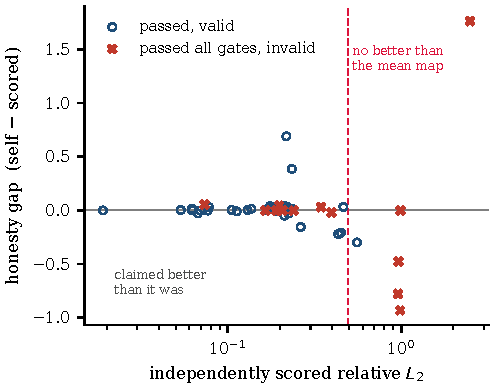
\includegraphics[width=0.52\textwidth]{figures/fig_verification}
\caption{The verification plane. Every point passed every contract gate.
Crosses are physically invalid artifacts; the dashed line is the mean-map
baseline. Large honesty gaps and invalid artifacts are largely different runs.}
\label{fig:verif}
\end{figure}

\section{Cost against accuracy}
\label{app:costfig}

\begin{figure}[htbp]
\centering
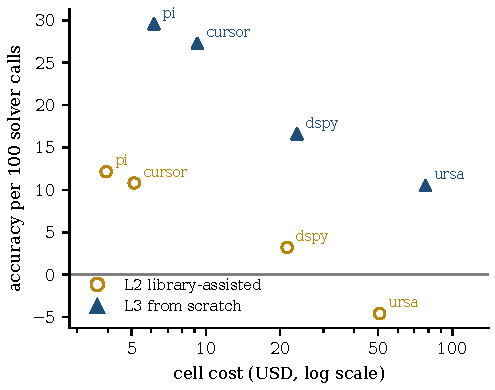
\includegraphics[width=0.52\textwidth]{figures/fig_cost}
\caption{What each cell's accuracy cost, at one model. A $13\times$ spread in
dollars buys no consistent advantage, and the most expensive substrate is the
least accurate at both access levels.}
\end{figure}

\section{The deliverable contract in full}
\label{app:gates}

\begin{table}[t]
\centering
\caption{The deliverable contract. \code{contract.passed} is the flat
\textsc{and} of all gates: no weighting, no partial credit. The scoring
subprocess is stripped of provider credentials, so \code{predict.py} must work
offline, and runs in its own process group so a timeout reaps the solver
children too.}
\label{tab:gates}
\small
\begin{tabular}{@{}ll@{}}
\toprule
\textbf{Gate} & \textbf{What it checks} \\
\midrule
\code{artifact:report.json} & present and non-empty \\
\code{artifact:predict.py}  & present and non-empty \\
\code{artifact:README.md}   & present and non-empty \\
\code{report\_parses}       & \code{report.json} is valid JSON \\
\code{report\_keys}         & \code{n\_solves\_\{attempted,succeeded\}} and \\
                            & \code{metrics.\{test,baseline\}\_rel\_l2.\{mean,median,p90\}} present \\
\code{no\_autotokamak\_import} & \Lthree{} only --- no workspace \code{.py} imports the platform \\
                            & library, by regex over plain imports, \code{importlib}, \code{\_\_import\_\_} \\
\code{predict\_runs}        & \code{python predict.py -{}-input params.json -{}-output pred.npz} exits 0 \\
\code{predict\_shape}       & returned \code{psi} is $(N, 96, 64)$ \\
\code{predict\_grid}        & returned \code{R}, \code{Z} match the frozen axes to $10^{-9}$ \\
\bottomrule
\end{tabular}
\end{table}

\section{Frozen assets}
\label{app:assets}

\begin{itemize}
\item \code{benchmarks/assets/eval\_grid.json} --- the frozen evaluation grid:
  64 points in $\Rgrid \in [0.15, 0.80]$\,m and 96 in $\Zgrid \in [-0.40,
  0.40]$\,m, both \code{linspace}. Flux arrays are stored $(N, 96, 64)$, that
  is $(N, n_Z, n_R)$.
\item \code{benchmarks/assets/test\_params.json} --- the 60 held-out parameter
  vectors, generated with seed \code{20260809}. SHA-256
  \code{d10a3651...d17b480}.
\item \code{benchmarks/assets/test\_set.h5} --- ground-truth flux fields, all 60
  solves converged; $80.46\%$ of grid points are NaN, outside the plasma.
  Provenance attributes record the stamp time, the solver version (26.6), the
  SHA-256 of both the parameter file and the grid, the sweep configuration and
  its hash, and the scoring epoch (\code{2026-08-18}). Never regenerated; every
  archived score is relative to it.
\item \code{benchmarks/assets/prices.json} --- the dated price table behind
  every derived cost figure, so a published dollar amount is traceable to the
  rates it was computed with.
\item \code{benchmarks/tasks/*.yaml} --- the task specifications.
\end{itemize}

\section{The task text, and the \texorpdfstring{\Ltwo{}/\Lthree{}}{L2/L3} difference}
\label{app:tasktext}

The \Lthree{} problem statement is reproduced verbatim below. The \Ltwo{} text
is byte-identical to it except for the ten hunks that follow, every one of which
concerns access level: the title, the description of the solver, the three
pipeline steps where the library would be used, the workspace and environment
bullets, the single-\code{OFT\_env} advice, and the constraints block. The
parameter ranges, the budget, the stopping criterion, the evaluation interface,
all five deliverables, the ``do not fabricate metrics'' paragraph and the three
process gates are identical.

\subsection{\Lthree{} problem statement (verbatim)}
% generated by tools/render_paper_tables.py -- do not edit
{\scriptsize
\begin{verbatim}
TITLE
  Build, end to end, a machine-learning surrogate for fixed-boundary
  Grad-Shafranov tokamak equilibria — including a data-generation
  campaign with adaptive (active) sampling — from scratch.

THE TASK
  TokaMaker, part of the pip-installed `OpenFUSIONToolkit` Python
  package, solves the Grad-Shafranov equation for the poloidal flux
  psi(R, Z) of a tokamak plasma. You will use it as your ground-truth
  physics solver.

  Consider fixed-boundary equilibria of D-shaped plasmas described by
  5 input parameters, with TokaMaker's default pressure/current
  profile shapes:

    r0    : major radius        [m]   in [0.35, 0.55]
    a     : minor radius        [m]   in [0.10, 0.20]
    kappa : elongation          [-]   in [1.0, 1.6]
    delta : triangularity       [-]   in [0.0, 0.4]
    Ip    : plasma current      [A]   in [80e3, 200e3]
    (plasma centered at z0 = 0)

  Your job, in full:
    1. Learn how to drive TokaMaker for fixed-boundary solves (mesh a
       D-shaped last-closed-flux-surface, solve, extract psi). Choose
       your own numerical resolution; a single solve should take
       seconds, not minutes.
    2. Design and run a DATA-GENERATION CAMPAIGN structured as an
       initial space-filling design of AT MOST 150 solves followed by UP TO 3 ADAPTIVE
       (ACTIVE-SAMPLING) ROUNDS of EXACTLY 100 new solver runs each
       (failed/unconverged solves count against a round's 100).
       A one-shot space-filling or random design alone is NOT
       sufficient: each round's 100 new solver evaluations must be
       chosen ADAPTIVELY, informed by the current model or data (your
       strategy — e.g. uncertainty, model error, disagreement,
       anything you can justify). STOPPING CRITERION: keep a held-out
       VALIDATION set (separate from the final test set of step 4,
       which must never influence the campaign); after each round,
       retrain your surrogate and stop the campaign early once its
       validation error is reduced by at least 70% relative to the
       mean-predictor baseline (a model that always predicts the
       training-set mean psi map), i.e. val_error <= 0.30 *
       baseline_error. Otherwise continue to the 3-round cap. Log
       every acquisition decision (which point, when, why) and each
       round's validation error vs baseline to an acquisition log
       file.
    3. Train an ML surrogate mapping the 5 parameters to the PHYSICAL
       poloidal flux psi(R, Z) in Webers (not a normalized flux).
       Model family, input/output representation, and training
       procedure are entirely your choice.
    4. Evaluate honestly on a held-out test set of AT LEAST 20 solver
       runs at uniformly random parameters (fixed recorded seed),
       generated independently and never used for training, model
       selection, or acquisition.
    5. Report results and analyze whether your adaptive sampling
       actually helped (e.g. versus the model trained on the initial
       design only, or any comparison you can defend).

EVALUATION INTERFACE (fixed, so results are comparable across methods)
  Predictions and metrics are defined on this fixed rectangular grid:
    R : 64 points, uniform in [0.15, 0.80] m
    Z : 96 points, uniform in [-0.40, 0.40] m
  psi arrays are shaped (96, 64) = (nZ, nR). Grid points outside the
  plasma boundary carry NaN; all metrics are computed only where the
  ground truth is finite.

  Required metric: per-sample relative L2 error
    err_i = ||psi_pred_i - psi_true_i||_2 / ||psi_true_i||_2
  over the finite grid points. Report mean, median, and 90th
  percentile over the test set, and the same numbers for a trivial
  baseline (predict the training-set mean psi) so the surrogate's
  value is evident.

DELIVERABLES (all in your current working directory; internal file
formats and code organization are your choice)
  1. Your pipeline code, runnable end to end by one documented entry
     command.
  2. The dataset(s) you generated, plus the acquisition log.
  3. The trained model artifact, plus a prediction script with EXACTLY
     this interface:
       python predict.py --input params.json --output pred.npz
     where params.json is a JSON list of objects with keys
     r0, a, kappa, delta, Ip, and pred.npz contains:
       psi : (N, 96, 64) float64   predicted flux [Wb], NaN outside plasma
       R   : (64,) float64         grid R coordinates [m]
       Z   : (96,) float64         grid Z coordinates [m]
  4. report.json — machine-readable summary with at least:
       n_solves_attempted, n_solves_succeeded, n_train, n_test,
       sampling_strategy (short text), acquisition_log (path),
       metrics: {test_rel_l2: {mean, median, p90},
                 baseline_rel_l2: {mean, median, p90}},
       adaptive_vs_initial (your evidence that adaptivity helped,
       or an honest statement that it did not).
  5. README.md — your design, why you chose it, how to run, results.

  You MUST actually run the full campaign and training within this
  session and verify every deliverable exists before declaring done.
  Report failures honestly in report.json/README; do not fabricate
  metrics.

ENVIRONMENT FACTS
  * Your current working directory IS your workspace. Create all files
    here. Do not read, copy, or import code from the surrounding
    repository. In particular the Python environment contains an
    installed package called `autotokamak` that solves a related
    problem — importing it, reading its source, or reusing its
    artifacts is FORBIDDEN: this is a from-scratch capability test,
    and only `OpenFUSIONToolkit` may be used for physics.
  * `python` resolves to a Python 3.11 venv that already has:
    numpy, scipy, h5py, matplotlib, pyyaml, scikit-learn, torch,
    optuna, OpenFUSIONToolkit. Nothing may be installed.
  * A read-only `./OpenFUSIONToolkit/` symlink to the full OFT
    source tree is present in your workspace. BEFORE writing any
    solver or meshing code, study the worked TokaMaker examples
    under `OpenFUSIONToolkit/src/examples/TokaMaker/` (the
    `fixed_boundary/` example is directly relevant) and follow the
    workflow they demonstrate rather than inventing your own
    solver-facing plumbing.
  * TokaMaker limitation: only ONE `OFT_env` may ever be created per
    Python process. Structure your code so the environment object is
    created once and reused across all solves in a process, or run
    solves in child processes.

CONSTRAINTS
  * MESHING MILESTONE (mandatory, before any campaign code): locate
    the fixed-boundary example under
    `OpenFUSIONToolkit/src/examples/TokaMaker/`, reproduce its
    mesh-and-solve workflow as a standalone script in your workspace,
    run it, and verify it produces finite psi values. Only then
    generalize it to your parameterized D-shape. Do not design your
    own meshing approach when the examples demonstrate one.
  * Do NOT construct the computational mesh yourself (e.g. via scipy
    Delaunay) and pass raw triangles to the solver — TokaMaker
    validates mesh topology and will reject hand-built
    triangulations. Use the meshing route the OFT examples use.
  * PILOT GATE (mandatory): before the campaign, run a pilot of at
    least 20 solves at random parameters. If the success rate is
    below 50%, STOP, diagnose the per-failure error messages, fix,
    and re-run the pilot. Never start the 100-solve rounds while the
    pilot is failing.
  * STORAGE VALIDATION GATE (mandatory): a solver run may be counted
    as successful ONLY after its stored artifact has been re-loaded
    from disk and verified: the saved psi grid must contain a nonzero
    fraction of finite values. Apply this check to every batch you
    write. A stored all-NaN psi grid is a FAILED solve regardless of
    solver exit status, and your reported success counts must be based
    on validated stored artifacts, not solver return codes.
  * DELIVERABLE SELF-TEST (mandatory, before declaring done): in a
    fresh Python process, run the exact documented command for each
    deliverable — including `python predict.py --input <sample params>
    --output <out>` — and verify the output loads with the required
    shapes and finite values. If any deliverable fails its own
    interface test, fix it and re-test. Code you have not re-run after
    your last edit does not count as verified.
  * Do not run `pip install` or modify the environment.
  * Do not call `git`.
  * Do not prompt for user input; the task is fully autonomous.
  * If errors arise, debug, fix your code, and re-run. Stay within
    the campaign structure above (at most 3 adaptive rounds x 100
    solves, plus the initial design and validation/test sets) across
    ALL attempts that reach the solver.
\end{verbatim}
}


\subsection{Diff from the \Ltwo{} statement}
% generated by tools/render_paper_tables.py -- do not edit
% 10 hunks
{\scriptsize
\begin{verbatim}
--- L2_mini_v3
+++ L3_mini_v3
@@ -4,2 +4 @@
-  campaign with adaptive (active) sampling — using the installed
-  `autotokamak` platform library wherever it helps.
+  campaign with adaptive (active) sampling — from scratch.
@@ -10,2 +9,2 @@
-  psi(R, Z) of a tokamak plasma. It is your ground-truth physics
-  solver, and the installed `autotokamak` package already wraps it.
+  psi(R, Z) of a tokamak plasma. You will use it as your ground-truth
+  physics solver.
@@ -25,4 +24,3 @@
-    1. Drive the solver for fixed-boundary solves. You may use
-       `autotokamak.data.sweep.run_sweep` (config-driven sweeps; also
-       accepts an explicit (N, 5) sample matrix), or go through
-       `autotokamak.core` directly. A single solve should take
+    1. Learn how to drive TokaMaker for fixed-boundary solves (mesh a
+       D-shaped last-closed-flux-surface, solve, extract psi). Choose
+       your own numerical resolution; a single solve should take
@@ -36,13 +34,13 @@
-       chosen ADAPTIVELY, informed by the current model or data
-       (`autotokamak.data.acquire` implements residual-UCB and PCA-GP
-       variance acquisition you may reuse, or bring your own).
-       STOPPING CRITERION: keep a held-out VALIDATION set (separate
-       from the final test set of step 4, which must never influence
-       the campaign); after each round, retrain your surrogate and
-       stop the campaign early once its validation error is reduced
-       by at least 70% relative to the mean-predictor baseline (a
-       model that always predicts the training-set mean psi map),
-       i.e. val_error <= 0.30 * baseline_error. Otherwise continue to
-       the 3-round cap. Log every acquisition decision (which point,
-       when, why) and each round's validation error vs baseline to an
-       acquisition log file.
+       chosen ADAPTIVELY, informed by the current model or data (your
+       strategy — e.g. uncertainty, model error, disagreement,
+       anything you can justify). STOPPING CRITERION: keep a held-out
+       VALIDATION set (separate from the final test set of step 4,
+       which must never influence the campaign); after each round,
+       retrain your surrogate and stop the campaign early once its
+       validation error is reduced by at least 70% relative to the
+       mean-predictor baseline (a model that always predicts the
+       training-set mean psi map), i.e. val_error <= 0.30 *
+       baseline_error. Otherwise continue to the 3-round cap. Log
+       every acquisition decision (which point, when, why) and each
+       round's validation error vs baseline to an acquisition log
+       file.
@@ -51,4 +49,2 @@
-       `autotokamak.surrogate` provides dataset loading, PCA
-       reduction, a model zoo (GP, kernel ridge, polynomial ridge,
-       MLP), and Optuna search; model family and representation
-       remain entirely your choice.
+       Model family, input/output representation, and training
+       procedure are entirely your choice.
@@ -107 +103,6 @@
-    here.
+    here. Do not read, copy, or import code from the surrounding
+    repository. In particular the Python environment contains an
+    installed package called `autotokamak` that solves a related
+    problem — importing it, reading its source, or reusing its
+    artifacts is FORBIDDEN: this is a from-scratch capability test,
+    and only `OpenFUSIONToolkit` may be used for physics.
@@ -110,8 +111,8 @@
-    optuna, OpenFUSIONToolkit, and the `autotokamak` platform library
-    (importable; using it is ALLOWED and RECOMMENDED — that is the
-    point of this condition). Nothing may be installed.
-  * Useful autotokamak entry points: `autotokamak.data.sweep.run_sweep`
-    (sweep or explicit-matrix solves → HDF5),
-    `autotokamak.data.acquire` (acquisition strategies),
-    `autotokamak.surrogate.dataset/reduce/zoo/optuna_search/automl_loop`
-    (loading, PCA, model factories, search). Read their docstrings.
+    optuna, OpenFUSIONToolkit. Nothing may be installed.
+  * A read-only `./OpenFUSIONToolkit/` symlink to the full OFT
+    source tree is present in your workspace. BEFORE writing any
+    solver or meshing code, study the worked TokaMaker examples
+    under `OpenFUSIONToolkit/src/examples/TokaMaker/` (the
+    `fixed_boundary/` example is directly relevant) and follow the
+    workflow they demonstrate rather than inventing your own
+    solver-facing plumbing.
@@ -119,4 +120,3 @@
-    Python process. `autotokamak.core.solver.make_solver` handles
-    reuse via its `env=` argument; if you bypass autotokamak, create
-    the environment object once and reuse it, or run solves in child
-    processes.
+    Python process. Structure your code so the environment object is
+    created once and reused across all solves in a process, or run
+    solves in child processes.
@@ -124,0 +125,11 @@
+  * MESHING MILESTONE (mandatory, before any campaign code): locate
+    the fixed-boundary example under
+    `OpenFUSIONToolkit/src/examples/TokaMaker/`, reproduce its
+    mesh-and-solve workflow as a standalone script in your workspace,
+    run it, and verify it produces finite psi values. Only then
+    generalize it to your parameterized D-shape. Do not design your
+    own meshing approach when the examples demonstrate one.
+  * Do NOT construct the computational mesh yourself (e.g. via scipy
+    Delaunay) and pass raw triangles to the solver — TokaMaker
+    validates mesh topology and will reject hand-built
+    triangulations. Use the meshing route the OFT examples use.
@@ -147,2 +157,0 @@
-  * Do not modify the installed autotokamak/OpenFUSIONToolkit
-    packages; use them as libraries.
\end{verbatim}
}


\section{Solution-shape cross comparison}
\label{app:shape}

Twelve questions, each answered from the code that plays the relevant role, with
\code{file:line} evidence recorded per run. Cells are abbreviated by level and
harness: \code{2c} is \Ltwo{}-\hn{cursor}, \code{3u} is \Lthree{}-\hn{ursa}, and
so on. A dash means the dimension is not answerable for that cell, which at
\Ltwo{} generally means the library owns that part of the pipeline.

\begin{center}
\scriptsize
% generated by tools/render_paper_tables.py -- do not edit
\begin{tabular}{@{}ll>{\raggedright\arraybackslash}p{0.44\textwidth}@{}}
\toprule
\textbf{Dimension} & \textbf{Cells} & \textbf{Modal value} \\
\midrule
code\_shape & 2c, 2p & \code{single\_script} \\
 & 2d & \code{14\_modules} \\
 & 2u & \code{15\_modules} \\
 & 3c & \code{8\_modules} \\
 & 3d & \code{11\_modules} \\
 & 3p & \code{9\_modules} \\
 & 3u & \code{7\_modules} \\
\addlinespace[2pt]
entry\_point & 2c, 2p, 3p & \code{2\_runnable\_scripts} \\
 & 2d, 3u & \code{10\_runnable\_scripts} \\
 & 2u & \code{9\_runnable\_scripts} \\
 & 3c & \code{3\_runnable\_scripts} \\
 & 3d & \code{7\_runnable\_scripts} \\
\addlinespace[2pt]
grid\_mapping & 2c, 2d, 2p, 2u & --- \\
 & 3c, 3d, 3p, 3u & \code{solver\_field\_eval} \\
\addlinespace[2pt]
mask\_rule & 2c, 2p, 3c, 3d, 3p & \code{lcfs\_polygon} \\
 & 2d, 2u & \code{training\_valid\_mask} \\
 & 3u & \code{lcfs\_polygon+training\_valid\_mask} \\
\addlinespace[2pt]
mesh\_route & 2c, 2u, 3c, 3d, 3p, 3u & \code{oft\_gs\_domain} \\
 & 2d, 2p & --- \\
\addlinespace[2pt]
oft\_env\_strategy & 2c, 2d, 2p, 2u & --- \\
 & 3c, 3d, 3p, 3u & \code{singleton\_reused} \\
\addlinespace[2pt]
self\_test & 2c, 2d, 2u, 3p, 3u & \code{subprocess\_reruns\_predict} \\
 & 2p, 3c, 3d & \code{imported\_not\_subprocessed} \\
\addlinespace[2pt]
solve\_isolation & 2c, 2d, 2p, 2u, 3c, 3d, 3u & \code{in\_process\_serial} \\
 & 3p & \code{subprocess\_per\_batch} \\
\addlinespace[2pt]
storage & 2c, 2p, 3c, 3p & \code{npz\_per\_solve+pickle} \\
 & 3d, 3u & \code{npz\_per\_solve+pickle+index} \\
 & 2d & \code{npz\_per\_solve+hdf5} \\
 & 2u & \code{npz\_per\_solve+hdf5+index} \\
\addlinespace[2pt]
leakage\_guard & 2c, 2d, 2p, 2u, 3c, 3d, 3p, 3u & \code{test\_absent\_from\_fitting\_functions} \\
\addlinespace[2pt]
pilot\_gate & 2c, 2d, 2p, 2u, 3c, 3d, 3p, 3u & \code{enforced} \\
\addlinespace[2pt]
storage\_validation & 2c, 2d, 2p, 2u, 3c, 3d, 3p, 3u & \code{reload\_and\_check\_finite} \\
\addlinespace[2pt]
\bottomrule
\end{tabular}

\end{center}

\section{Glossary of canonical values}
\label{app:glossary}

Every code printed in Table~\ref{tab:logic} and Appendix~\ref{app:shape}. A code
a reader has to guess at is not a measurement.

% generated by tools/render_paper_tables.py -- do not edit
\begin{description}[leftmargin=1.2em,style=nextline,font=\ttfamily\small]
\item[N\_modules] The pipeline is spread over N source files, none of them dominant; contrast \code{single\_script}.
\item[N\_runnable\_scripts] N files are runnable as programs. More than one means the documented single command is really a sequence.
\item[adaptive\_in\_name\_only] Every stated criterion names nothing but randomness: the round was labelled adaptive and was not.
\item[agree] The criterion stated in the log/report is the one the code computes.
\item[chain\_agreement] Share of a cell's replicates that chose the modal chain of methods — method reproducibility, which is not the same as score reproducibility.
\item[criterion\_switched] The acquisition criterion CHANGED between rounds — logic reacting to what it measured, rather than one fixed rule executed n times.
\item[deep\_ensemble] Several independently initialised models, averaged.
\item[enforced] A pilot runs and its success rate is compared against a threshold before the campaign proceeds — the task's 50\% pilot gate.
\item[evidence\_grounded] The round's validation error against baseline was recorded, so its choice can be checked against what was known at the time. An ungrounded round's reasoning is unfalsifiable.
\item[feasibility] Candidate choice weighted by whether solves there are expected to converge, steering away from regions with failed solves.
\item[gradient\_sensitivity] Points where the response is steep or curving — a sensitivity or Jacobian-driven criterion.
\item[hdf5] One HDF5 file holding many samples. Scales best and carries attributes/provenance, at the price of concurrent-write care.
\item[imported\_not\_subprocessed] predict.py is referenced but only imported or described, never run as the documented command. Code that works in the session's process and fails in a clean one is exactly what this misses.
\item[in\_process\_serial] Solves run one after another inside the driving process. Simplest, and the slowest: no parallelism, and one bad solve can poison the shared solver state.
\item[index] An index/manifest (CSV or JSONL) sits beside the arrays, listing every sample and its status. What makes a campaign resumable and auditable rather than a directory to be re-scanned.
\item[kernel\_ridge] Kernel ridge regression — a GP's mean without its variance.
\item[lcfs\_polygon] A grid point is inside the plasma iff it lies within the LCFS polygon — point-in-polygon against the D-shape boundary, whatever the helper is called (contains\_points, \_points\_in\_poly, inside\_lcfs\_mask). Geometric, per sample, and independent of the surrogate's own output.
\item[lhs] Latin hypercube: stratified in every dimension at once.
\item[mc\_dropout] Dropout left active at inference and sampled repeatedly — an ensemble's spread at one model's training cost.
\item[mismatch] The stated criterion and the implemented one have nothing in common. The strongest available signal that a run's account of itself is wrong.
\item[mlp\_torch] A hand-written PyTorch MLP. The most common choice in this corpus, usually mapping 5 parameters to PCA coefficients.
\item[model\_informed] The function that chooses points actually calls the surrogate. A model-derived criterion that never does is not one, whatever it is named.
\item[npz\_per\_solve] One compressed .npz per solved sample.
\item[oft\_gs\_domain] Meshed through OFT's own API (gs\_Domain / define\_region / build\_mesh) as the worked examples do. What the task's meshing milestone asks for, and what TokaMaker's topology checks accept.
\item[partial] Stated and implemented criteria overlap but do not match: one side names a component the other never does — see claimed-but-not-computed.
\item[pickle] Python-pickled objects (pickle/joblib/torch.save) — usually the model artifact rather than the dataset.
\item[prose\_only] A method named in the README or report.json that the code never evidences.
\item[random] Points drawn uniformly at random. As the CANDIDATE POOL this is normal and harmless; as the selection criterion it means the round was adaptive in name only.
\item[reload\_and\_check\_finite] A function both re-loads a written artifact and checks its finite fraction — the task's storage-validation gate, actually implemented. This is the check that catches an all-NaN grid stored as a success.
\item[residual\_ucb] Points are targeted where the model is MEASURABLY wrong — an error model fit on residuals or out-of-fold error, often with a UCB trade-off between exploiting known weakness and exploring. Uses measurement rather than the model's self-assessment, which can be confidently wrong.
\item[round\_cap] Stop because the 3-round cap was reached.
\item[single\_script] The whole pipeline is one or two files.
\item[singleton\_reused] One OFT\_env is built once and handed out on every call — a cached module global, a class guarding construction, or an lru\_cache. Honours OFT's one-env-per-process limit in the simplest way, at the cost of keeping every solve in one process: a solver crash takes the campaign with it.
\item[sobol] A Sobol low-discrepancy sequence — quasi-random, extensible.
\item[solver\_field\_eval] psi is read on the frozen 64x96 grid through the solver's own finite-element interpolator (get\_field\_eval). Evaluates the FE basis directly, so no second interpolation error is introduced.
\item[space\_filling] Purely geometric coverage of the input box: farthest-point/maximin, distance to the existing training set, k-means. Needs no model at all — which makes it robust, and makes it NOT adaptive in the sense of reacting to what was learned.
\item[stop\_threshold\_met] The campaign ended with the task's 70\% criterion satisfied — the intended way to finish early.
\item[stop\_unexplained] The campaign ended and no per-round validation error was recorded, so why it stopped cannot be read from the artifacts at all.
\item[stop\_without\_threshold] The campaign ended although validation error had NOT reached 0.30x baseline: the round cap, a budget, or a timeout ended it, not the stopping rule.
\item[subprocess\_per\_batch] The driver shells out (usually to its own script) to run a batch. Insulates solver state between batches and survives a hard crash; pays process start-up and serialises through files.
\item[subprocess\_reruns\_predict] Something in the workspace invokes predict.py as a subprocess with the contract CLI — the task's deliverable self-test, in a fresh process, which is the only way to catch an import-order or global-state dependency.
\item[test\_absent\_from\_fitting\_functions] No function that calls .fit()/backward()/optimizer.step() references a test path or array. Necessary, not sufficient: the task also forbids the test set influencing model SELECTION and ACQUISITION, which this check cannot see.
\item[top\_k] The highest-scoring candidates are taken (argsort/topk).
\item[training\_valid\_mask] The predictor masks with a valid-pixel mask derived from the training data (e.g. pixels finite in training). Cheap and stable, but the mask cannot adapt to a geometry unlike those seen in training — the same family of defect as the run that passed 9/9 gates while predicting plasma in vacuum.
\item[uncertainty] Points are ranked by the model's own predictive spread, without the record saying where that spread comes from. The family term; the two entries below are its specific forms.
\item[uncertainty\_ensemble] Spread across an ENSEMBLE of models (deep ensemble, bootstrap, or MC-dropout samples) — 'query by committee'. Needs no probabilistic model, and its quality depends entirely on the members disagreeing for real rather than sharing an initialisation.
\item[uncertainty\_gp] Posterior variance of a Gaussian process (or an acquisition built on it, e.g. expected improvement). Principled and calibrated where the GP's kernel assumptions hold; costly as the dataset grows.
\item[uniform\_random] Independent uniform draws, with no stratification.
\item[unverifiable\_from\_code] No function that chooses points could be classified, so the stated criterion can be neither confirmed nor contradicted.
\item[val\_threshold\_70pct] The task's own rule: stop once validation error is at most 0.30x the mean-predictor baseline, i.e. a 70\% reduction.
\end{description}

